\documentclass[UTF8,twoside,fontset=none,heading=true,scheme=chinese]{ctexart}

% 设置页边距
\usepackage{geometry}
\geometry{top=2.2cm,bottom=2.2cm,left=1.95cm,right=1.95cm,hoffset=0cm}

%设置页眉页脚
\pagestyle{plain}
\pagenumbering{arabic}
%\usepackage{fancyhdr}
%\fancyhf{}
%\fancyfoot[C]{\xiaowu \thepage}

% 设置行间距
\linespread{1.3}\selectfont

%设置字体
\usepackage{fontspec,xeCJK}
%设置英文字体
\setmainfont{Times New Roman} %衬线字体
\setsansfont{Helvetica Neue}  %非衬线字体
\setmonofont{Source Code Pro} %等宽字体
%设置中文字体
\newcommand\FONTsongti{Source Han Serif CN}         %思源宋体
\newcommand\FONTheiti{Source Han Sans CN Medium}    %思源黑体
\newcommand\FONTkaishu{FZKai-Z03S}                  %方正简体楷(无版权)
\newcommand\FONTfangsong{FZFangSong-Z02S}           %方正仿宋(无版权),方正隶书有版权
\setCJKfamilyfont{songti}{\FONTsongti}
\setCJKfamilyfont{heiti}{\FONTheiti}
\setCJKfamilyfont{kaishu}{\FONTkaishu}
\setCJKfamilyfont{fangsong}{\FONTfangsong}
\newcommand\songti{\CJKfamily{songti}}
\newcommand\heiti{\CJKfamily{heiti}}
\newcommand\kaishu{\CJKfamily{kaishu}}
\newcommand\fangsong{\CJKfamily{fangsong}}
\setCJKmainfont[BoldFont=\FONTheiti, ItalicFont=\FONTkaishu]{\FONTsongti}   %加粗为黑体,斜为楷书,正文为宋体
\setCJKsansfont{\FONTheiti}
\setCJKmonofont{\FONTfangsong}

%设置字号
\usepackage{ctexsize,type1cm}
\newcommand{\yihao}{\fontsize{26pt}{39pt}\selectfont}
\newcommand{\xiaoyi}{\fontsize{24pt}{36pt}\selectfont}   
\newcommand{\erhao}{\fontsize{22pt}{33pt}\selectfont}          
\newcommand{\xiaoer}{\fontsize{18pt}{27pt}\selectfont}          
\newcommand{\sanhao}{\fontsize{16pt}{24pt}\selectfont}        
\newcommand{\xiaosan}{\fontsize{15pt}{22.5pt}\selectfont}        
\newcommand{\sihao}{\fontsize{14pt}{21pt}\selectfont}            
\newcommand{\xiaosi}{\fontsize{12pt}{18pt}\selectfont}            
\newcommand{\wuhao}{\fontsize{10.5pt}{15.75pt}\selectfont}
\newcommand{\xiaowu}{\fontsize{9pt}{13.5pt}\selectfont}    
\newcommand{\liuhao}{\fontsize{7.5pt}{11.25pt}\selectfont}

%使用希腊字符
%\usepackage[greek,english]{babel}

%使用公式,表格,图片
\usepackage{mathtools,amsmath,graphicx,array}

%设置参考文献
\bibliographystyle{plain}

\ctexset {
    autoindent=false,
    bibname={参考文献:},
    section={
        format={\raggedright \sihao \textbf},
        number={\arabic{section}},
        afterindent=true,
        beforeskip=0pt,
        afterskip=0pt,
        fixskip=false
    },
}

%使用代码排版包
\usepackage{listings}
\usepackage{color}
\lstset{%
    frame=shadowbox,
    extendedchars=false,            % shutdown no-ACSII compatible
    language=python,
    basicstyle=\wuhao,              % 字体大小设置
    tabsize=4,
    numbers=left,
    numberstyle=\small,              % 行号字体设置
    stepnumber=1,                   % 行号距离设置,1代表每行加行号
    numbersep=8pt,                  % 行号和代码距离设置
    backgroundcolor=\color{white},
    showspaces=false,               % show spaces adding particular underscores
    showstringspaces=false,         % 使用下划线连接字符串
    showtabs=false,
    frame=single,                   % 给代码加边框
    captionpos=b,                   % sets the caption-position to bottom
    breaklines=true,                % 自动换行设置
    breakatwhitespace=false,        % sets if automatic breaks should only happen at whitespace
    escapeinside={\%*}{*)},         % if you want to add a comment within your code
    xleftmargin=2em,                % 设置左边距,宽度默认是与页芯等宽的
    xrightmargin=2em,               % 设置右边距,宽度默认是与页芯等宽的
    aboveskip=1em                   % 设置上边距
}

%设置自定义变量
\newcommand\degree{^\cire}

%正文区(文稿区)
\begin{document}\wuhao

    \begin{center}
        \vspace{6pt}
        \erhao \textbf{
        数据二分类实验
        }
        \vspace{8pt}
    \end{center}

    \section{实验目标}
    \noindent 给定一个可二分类的二维数据集,通过使用机器学习方法求出一个模型(即分类直线),具有良好的泛化能力,
    对测试集内的数据也进行正确分类。

    \section{实验结构}
    \noindent AI-homework\quad 项目文件夹 \\    
    -------+ main.py  \qquad 总实验 \\
    -------+ data.py  \qquad 数据集准备 \\  
    -------+ data\_visual.py  \qquad 数据可视化 \\
    -------+ perceptron\_algor.py  \qquad 感知机算法 \\
    -------+ choose\_model.py  \qquad 选择最佳模型 \\
    -------+ svm\_algor.py  \qquad 支持向量机算法 \\

    \section{人员分配}
    \noindent 杨军典:实验设计。对实验的目标、结构、可行性等方面进行分析、制定,对python语言进行支持。\\
    熊春艳:准备数据集。对实验所需的数据集构造、处理、标记,将结果返回给main文件。\\
    周世年:感知机算法设计。设计训练集的感知机算法,并在测试集上测试,可视化并分析结果。\\
    尚大伟:SVM算法设计。采用SVM算法对原始数据进行分类测试,可视化并分析结果。 \\
    司远:辅助ppt制作。

    \section{实验流程}
    \noindent 如图所示

    \section{数据集准备}
    \noindent 输入:数据集个数  \\
    输出:标记过的可二分类的训练集和测试集(数量比例4:1) \\
    设计数据集数据结构:$dataSets=[ [],[],...,[] ]$,整体是一个列表,其中每个数据元素点也是一个列表。 \\
    数据元素点列表结构为1*3,其中最后一个元素代表标记值。    \\
    设计算法:  \\
    1、随机产生N组2维数据点(代表平面上的一个点),限定所有数据点的x和y轴范围均在[-100,100]。    \\
       即生成一个$N*2$的矩阵,其中每个元素的值范围都在[-100, 100]。    \\
    2、设定标记模型:人为设定分类线为 $x-y=0$,法向量为$w=[1, -1]$,$b=0$。   \\
    3、标记数据点:将第1步产生的数据点根据第2步的模型进行标记正负,正实例为1,负实例为-1。   \\
    4、将标记过的数据永久保存成磁盘上的csv文件。
    4、将在内存中标记过的数据集按照4:1的比例分割为训练集和测试集进行返回。

    \section{感知机算法}
    \noindent 输入:训练集数据,K折参数 \\ 输出:模型(分类直线参数和模型得分) \\
    因为训练集的数量较少和为了提高泛化能力,将训练集按照K折交叉验证的方法进行模型的训练。\\
    每折采用感知机算法,即模型误分类数最小和随机梯度下降更新参数。
    最后返回每折的模型参数(直线的法向量和截距)和模型的验证分数。
    最佳模型取验证分数最小的模型参数。

    \section{可视化模型结果并分析}
    \noindent 某次实验结果中模型在可视化如图\ref{fig:per}所示。
    \begin{figure}[htb]
        \centering
        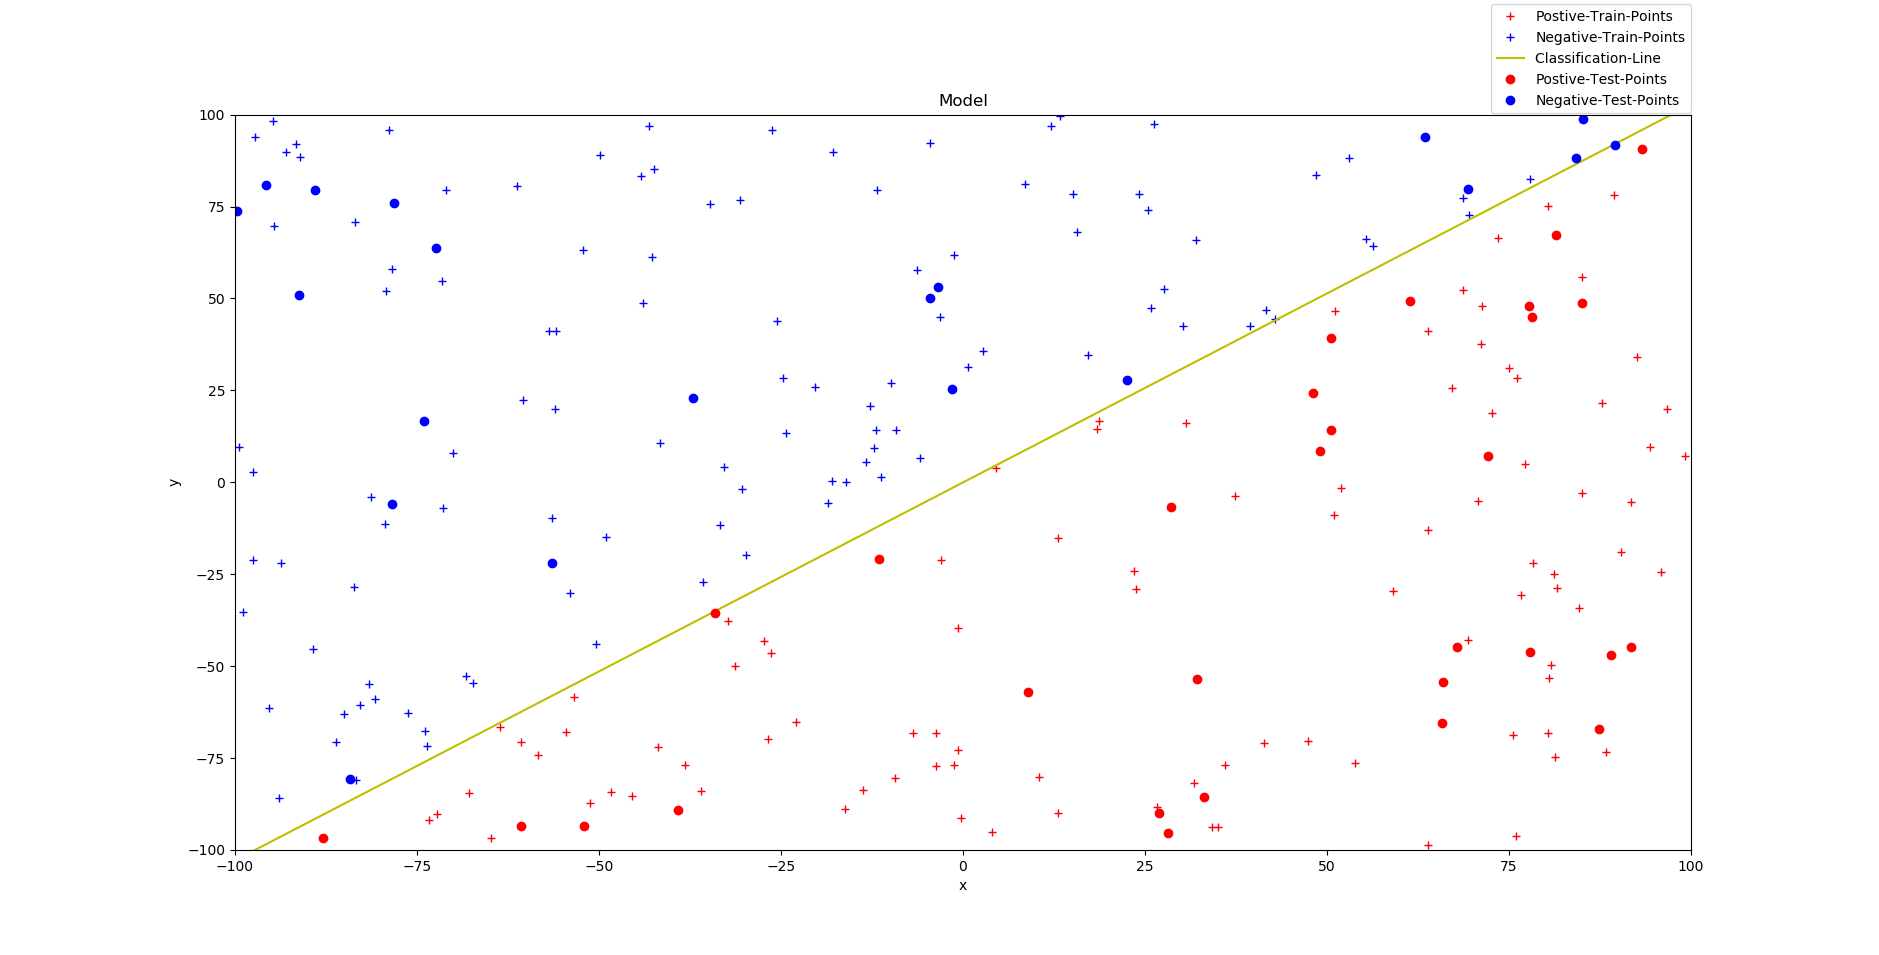
\includegraphics[scale=0.4]{../Model.png}
        \caption{感知机算法生成的模型可视化结果}
        \label{fig:per}
    \end{figure}
    由图\ref{fig:per}可以看出,模型对训练集和测试集的分类效果并不是非常好。分类线距离训练集中正负实例点的距离非常近。
    因此,考虑换一个策略,使用SVM算法使训练集中的数据类别间隔最大化,而且允许一定的误分类点。

    \section{支持向量机算法}
    \noindent 考虑到SVM中SMO算法比较复杂,而且有成熟的库模块可以使用。
    因此基于避免重复造轮子的考虑,直接使用scikit-learn库中的SVM算法模型,重点在于库API的使用和结果的分析。
    另外本模块不再使用之前的方法通过函数参数获得数据,而是换个思路使用pands来处理data.py中生成的csv数据。\\
    在同样的数据下数据可视化结果如图\ref{fig:svm}所示
    \begin{figure}[htb]
        \centering
        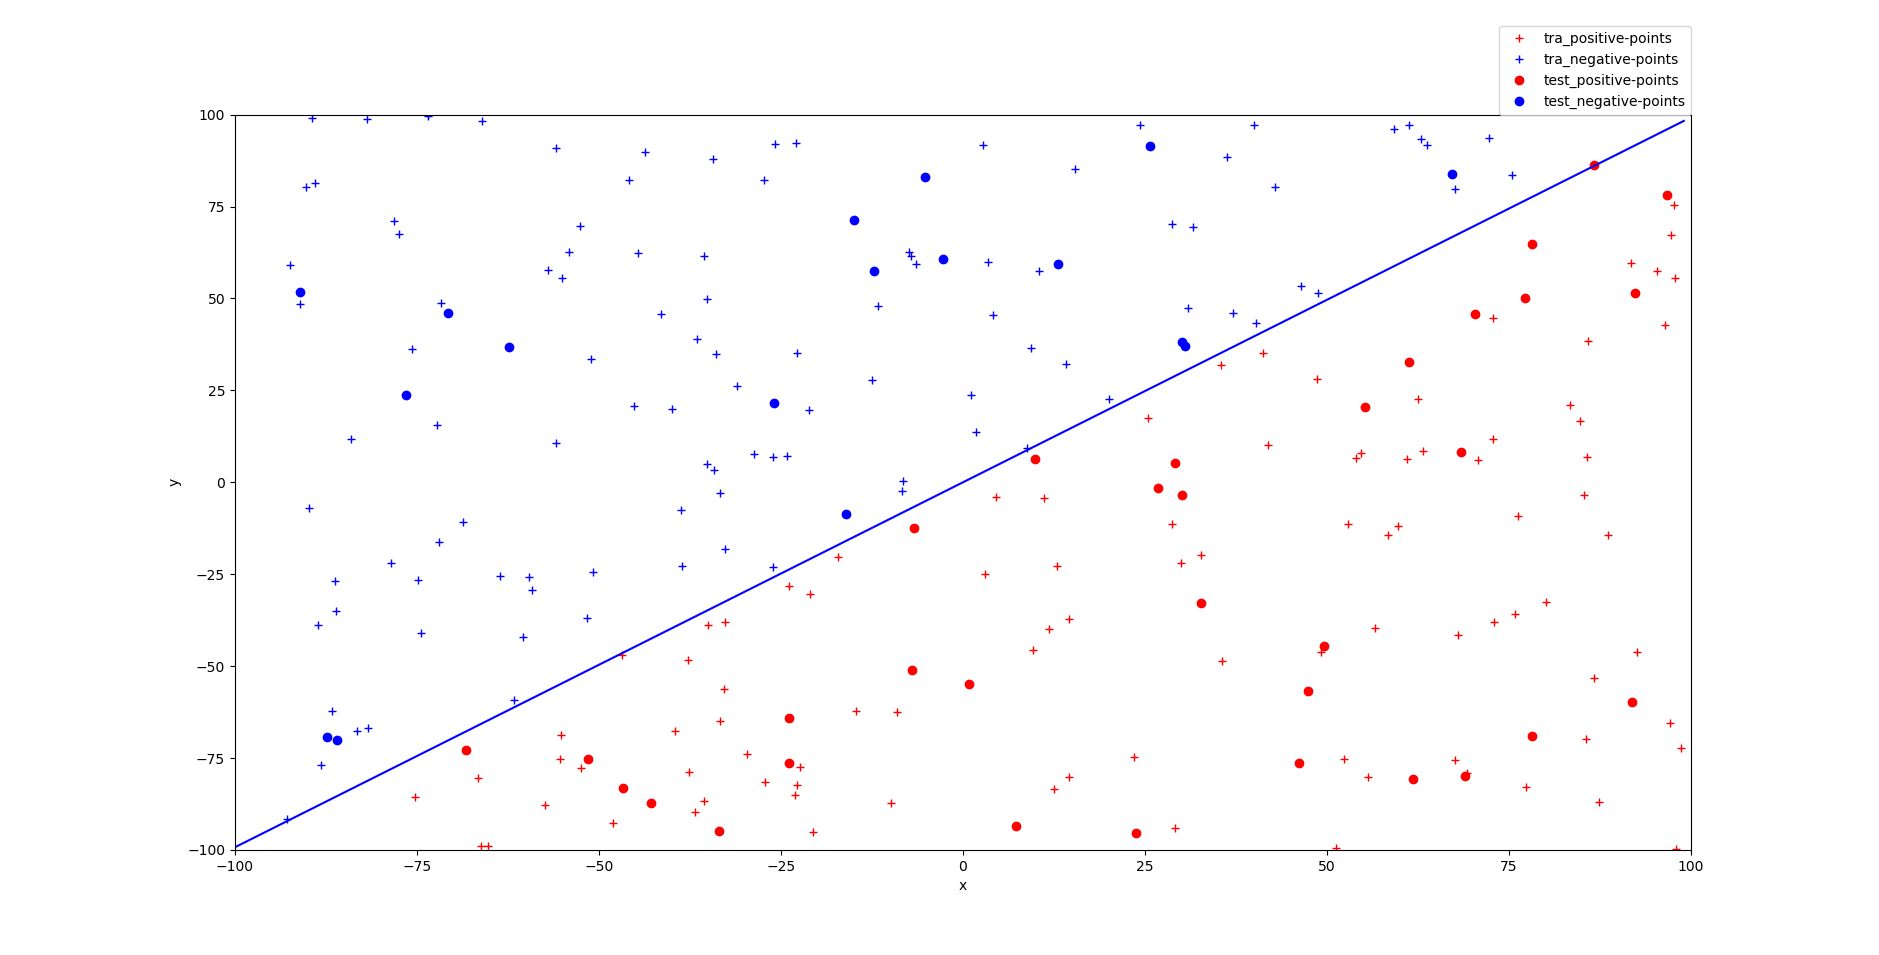
\includegraphics[scale=0.4]{../svm_model.png}
        \caption{SVM算法生成的模型可视化结果}
        \label{fig:svm}
    \end{figure}
    实验结果分析:从图\ref{fig:svm}可以看出,分类线直接比感知机算法得出的结果要更好,可以将测试集的数据正确分类。\\
    但是,同样存在一些问题,分类线与正负实例的距离过近。
    问题的源头来源于数据集,在data.py中,我们采用的是$0-1$均匀分布生成位于[0,1]之间的数据,然后将这些数据
    通过线性运算扩展区域到[-100,100]之内,均匀分布的特点造成了数据在直线$x-y=0$附近会出现这样的密集度问题,
    从而在直线附近会出现标记的正负实例点。因此造成上述所说的问题。

    \section{实验总结}
    \noindent 从上面的陈述中可以得出以下结论:\\
    1、数据的正确性对后续算法、模型的产生非常重要。一定要对原始数据进行一定的处理,包括去噪声、清洗等。如果输入算法的
    数据有问题,那么会对之后的结果分析产生非常大的干扰。\\
    2、一个问题通过不同的算法求解可以得出不同的结果,通过对结果的分析,找到不足的原因然后进行优化选择。

\end{document}
